\documentclass[11pt,a4paper]{article}
\usepackage[margin=21mm]{geometry}
\usepackage[T1]{fontenc}
\usepackage{lmodern,amsmath,amssymb,booktabs,array,longtable,graphicx,xcolor,hyperref,fancyhdr,microtype}
\usepackage{float}
\hypersetup{colorlinks=true,linkcolor=blue!55!black,urlcolor=blue!50!black,citecolor=blue!55!black}
\newcommand{\rhoF}{\rho_{\!f}}
\newcommand{\rhoE}{\rho_{\!E}}
\newcommand{\rhoM}{\rho_{\!m}}
\newcommand{\vswirl}{\mathbf{v}_{\!\boldsymbol{\circlearrowleft}}}
\newcommand{\dd}{\mathrm{d}}
\newcommand{\om}{\boldsymbol\omega}
\newcommand{\Gm}{\Gamma}
\newcommand{\rc}{r_c}
\newcommand{\X}{\mathbf X}
\newcommand{\q}{\mathbf q}
\newcommand{\vv}{\mathbf v}
\newcommand{\ec}{\mathcal E}
\newcommand{\NotRun}{\textsc{not run}}
\pagestyle{fancy}\fancyhf{}\fancyhead[L]{SST Research \quad VAM-5 $\times$ SST-17 $+$ SST-33/35}\fancyhead[R]{v0.3.0 DEVELOPMENT}\fancyfoot[C]{\thepage}\setlength{\headheight}{15pt}
\title{\textbf{SST Integrated Action v0.3.0}\\[0.5ex]\large Finite-Core Filament Diagnostics, Resonance Identifiability, and Thermodynamic Qualification}
\author{Versioned mathematical and numerical reconstruction of source manuscripts by O. Iskandarani\\\small SST-Workbench candidate research artifact; historical sources unchanged}
\date{20 October 2026 --- \textbf{DEVELOPMENT / NOT PHYSICALLY CERTIFIED}}
\begin{document}\maketitle
\begin{abstract}
This version extends the constrained Euler--director action of v0.2.0 with explicit, reproducible \emph{non-native} finite-core filament experiments for an unknotted ring $0_1$ and a torus trefoil $3_1$, a corrected normalized spectral-overlap model based on SST-35, and source-critical checks of the thermodynamic hypotheses in two SST-33 manuscripts. The computational method is an $O(N^2)$ regularized midpoint filament Biot--Savart approximation, not a full three-dimensional Euler solver, not the user's registered PKLSA backend, and not a self-consistent Euler--director dynamics. Fifty-five new local tests and forty-seven inherited v0.2.0 tests pass. The v0.3.0 results include short-time geometric drift, impulse convergence, synthetic spectral identifiability, and thermodynamic algebraic checks; \emph{none} establish photon propagation, Swirl-Clock proper-time dilation, equilibrium heat capacity, gravity, charge or quantized spin. A precise native-PKLSA input/source qualification contract is defined for future engine-controlled execution without representing surrogate results as physical certification.
\end{abstract}
\tableofcontents\clearpage
\section{Provenance, source audit and scope}
\begin{table}[H]\centering\small
\caption{Scope of the newly inspected manuscripts; source claims and their audited status are distinguished.}
\begin{tabular}{p{.29\linewidth}p{.33\linewidth}p{.30\linewidth}}\toprule
Source and page & Reusable mathematical element & Required caveat / repair \\\midrule
SST-33 Heat Transport (2026), pp. 3--7 \cite{SST33heat} & Off-diagonal coherence kernel, linewidth and thermal-bar design & $\kappa$ must be dimensionally normalized; coil chirality asymmetry requires an explicit odd coupling, not a symmetric Lorentzian alone \\
SST-33 HEAT Compare (2026), pp. 4--7 \cite{SST33compare} & Geometric strain $\epsilon$, harmonic energy curvature and a possible breathing coordinate & $T_{\rm swirl}=\Theta\epsilon$ is not equilibrium temperature; $C_V\propto T$ is not established by a single coherent oscillator \\
SST-35 Resonance Overlap (2026), pp. 1--5 \cite{SST35} & Voigt line profile; Fisher information, parameter fitting and optimal scan design & Correct factors for Gaussian and Lorentzian normalization; synthetic peak must not be labeled a measured vortex eigenmode \\
Previous v0.2.0 (2026) \cite{SSTv020} & Constrained material Euler action + independent transverse director action & The extra director stiffness and inertia are input data; free Maxwell mapping is not native Euler--photon closure \\\bottomrule
\end{tabular}\end{table}
The two published SST-33 abstracts discuss thermodynamic heat transport, but the first uses open-system density-matrix damping. Damping, the Born--Markov approximation and thermal gradients are \emph{not} consequences of the strictly inviscid Euler action. Neither thermodynamic paper supplies a source-native PKLSA flow solution. The SST-35 source contains a placeholder DOI and a non-committal link between its generic spectral kernel and SST modes. Its method is adopted as \emph{measurement mathematics}, not a fusion-yield or elementary-particle prediction.

\section{Physical hierarchy and inherited action}
Absolute background time $t$ is used throughout. The historical canonical numbers used here are
\begin{align}
\rc &=1.40897017\times10^{-15}\ \mathrm m,&
\lVert\vswirl\rVert &=1.09384563\times10^6\ \mathrm{m\,s^{-1}},\\
\rhoF&=7.0\times10^{-7}\ \mathrm{kg\,m^{-3}},&
\Gm&=2\pi\rc\lVert\vswirl\rVert=9.68361920349\times10^{-9}\ \mathrm{m^2\,s^{-1}},\\
\Omega_0&=\lVert\vswirl\rVert/\rc=7.76344065538\times10^{20}\ \mathrm{rad\,s^{-1}},&
\rhoE&=\rhoF\lVert\vswirl\rVert^2/2=4.18774\times10^5\ \mathrm{J\,m^{-3}},\\
\rhoM&=\rhoE/c^2,&\mathrm{d}t_{\rm ref}&=\rc^2/\Gm=2.05005680029\times10^{-22}\ \mathrm s.
\end{align}
Here $\Omega_0$ is a \emph{kinematic core-rate scale}, not a measured oscillation eigenfrequency; $\mathrm{d}t_{\rm ref}$ is a time unit, not a local proper-time tick. Numerical values from this manuscript cannot validate the constants from which they were constructed.

In v0.2.0 the material map $\X(\mathbf a,t)$, $F=\partial\X/\partial\mathbf a$, $J=\det F$, and director displacement $\q(\mathbf a,t)$ obey a proposed action \cite{SSTv020}
\begin{equation}
\mathcal A=\int\dd t\int\dd^3a\left[\frac{\rhoF}{2}|\dot\X|^2+\frac{\rho_d}{2}|\dot\q|^2-\frac K2|\nabla_{\!x}\times\q|^2+p(J-1)+\eta\nabla_{\!x}\cdot\q\right].
\end{equation}
The Euler limit is $\q=0$, $\eta=0$ and $J=1$. The frozen-reference director obeys
\begin{equation}
\partial_t^2\q-c_d^2\nabla^2\q=0,\qquad \nabla\cdot\q=0,\qquad c_d^2=K/\rho_d.
\end{equation}
This exact \emph{formal model limit} does not imply that an inviscid incompressible Euler medium has a finite shear modulus, nor does it predict $c$. We do not change this action in v0.3.0. Instead we qualify an independent filament-only diagnostic and identify the absent cross-coupling measurements.

\section{Explicit finite-core surrogate -- not native PKLSA}
\subsection{Registered target and executed stand-in}
The desired next step is the native PKLSA finite-core/Biot--Savart/Euler workflow. The required source code and exact runtime provider are \emph{not present in this package}; execution as though this had been found would break scientific provenance. To support near-term geometric diagnostics without misattribution, v0.3.0 uses a deliberately separate, transparent filament surrogate with periodic straight segments. The two initial geometries are
\begin{equation}
\frac{\X_{0_1}(\vartheta)}{\rc}=\begin{pmatrix}8\cos\vartheta\\8\sin\vartheta\\0\end{pmatrix},\qquad
\frac{\X_{3_1}(\vartheta)}{\rc}=\begin{pmatrix}(5+2\cos3\vartheta)\cos2\vartheta\\(5+2\cos3\vartheta)\sin2\vartheta\\2\sin3\vartheta\end{pmatrix}.
\end{equation}
These are \emph{synthetic seeds}, not certified knot-library production geometries. The right-hand formula is a torus trefoil of type $T(2,3)$, subject to orientation convention.
\begin{figure}[H]\centering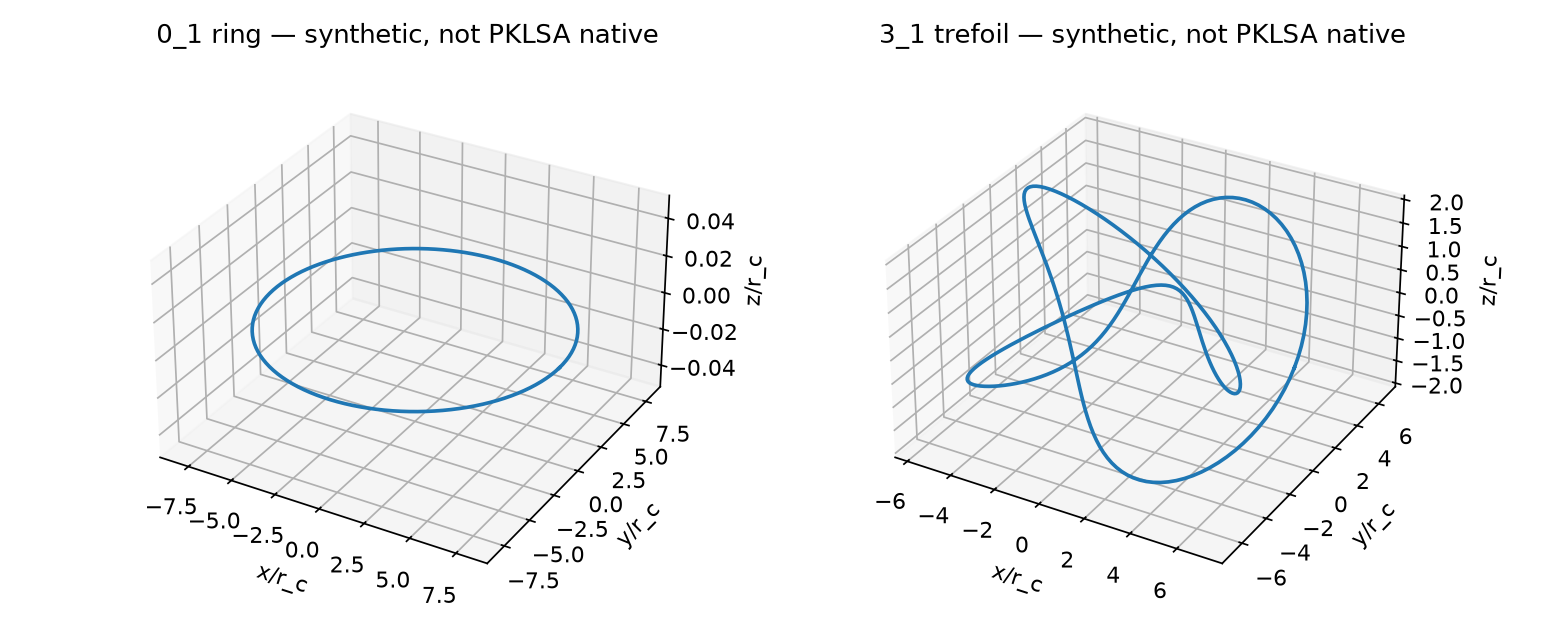
\includegraphics[width=\linewidth]{results/geometry.png}\caption{Geometry inputs in $r_c$ units; neither geometry has been imported from a native PKLSA asset.}\end{figure}

\subsection{Regularized segment-midpoint kernel}
Let dimensionless nodal coordinates be $\widehat\X_i=\X_i/\rc$, segment midpoints $\widehat{\mathbf m}_j=(\widehat\X_j+\widehat\X_{j+1})/2$, and $\Delta\widehat\X_j=\widehat\X_{j+1}-\widehat\X_j$. At unit normalized core cutoff $\widehat a=a/\rc=1$, the discretized self-induced speed is
\begin{equation}
\frac{\vv_i}{\Gm/\rc}=\frac1{4\pi}\sum_j\frac{\Delta\widehat\X_j\times(\widehat\X_i-\widehat{\mathbf m}_j)}{(|\widehat\X_i-\widehat{\mathbf m}_j|^2+\widehat a^2)^{3/2}}.
\label{eq:smoothed}
\end{equation}
This form approximates a regularized filament Biot--Savart law \cite{Saffman}; it is not an integration of the pressure-Poisson-constrained 3D Euler PDE. Finite thickness is encoded solely in the denominator and is not a resolved vorticity profile. RK4 moves the filament nodes without remeshing or collision detection. Long-time reconnection, Kelvin--Floquet spectra, vorticity divergence and fluid--director stress response are therefore not qualified.

Two diagnostics are computed in consistent units:
\begin{align}
\frac{E_{\rm fil}}{\rhoF\Gm^2\rc}&\equiv\frac1{8\pi}\sum_{ij}\frac{\Delta\widehat\X_i\cdot\Delta\widehat\X_j}{\sqrt{|\widehat{\mathbf m}_i-\widehat{\mathbf m}_j|^2+\widehat a^2}},\\
\frac{\mathbf I_{\rm fil}}{\rhoF\Gm\rc^2}&\equiv\frac12\sum_i\widehat\X_i\times\Delta\widehat\X_i.
\end{align}
$E_{\rm fil}$ is a \emph{regularized filament-energy proxy}. It excludes unspecified internal core energy, background subtraction, material director excitation and thermodynamic entropy. $\mathbf I_{\rm fil}$ is a filament hydrodynamic-impulse proxy. Neither is a confirmed SST particle mass.

\subsection{Executed numerical checks}
\begin{table}[H]\centering\caption{Ring calculation for $R/\rc=8$, $\widehat a=1$: geometric surrogate, not observed physical drift.}
\begin{tabular}{rccc}\toprule
$N$ & $\overline u_z/(\Gm/\rc)$ & $I_z/(\rhoF\Gm\rc^2)$ & analytic circle $I_z/(\rhoF\Gm\rc^2)$\\\midrule
64&0.02986130&200.73910&201.06193\\
128&0.03096395&200.98119&201.06193\\
256&0.03124595&201.04174&201.06193\\
512&see CSV&see CSV&201.06193\\\bottomrule
\end{tabular}\end{table}
At $N=256$, the nominal velocity conversion is $\overline u_z=2.14748\times10^5\ \mathrm{m\,s^{-1}}$. It is a result of the \emph{chosen} kernel and prescribed geometry, not an independently verified photon or particle speed. Short-time trefoil evolution with $N=96$ and $\Delta\widehat t=0.01$ for 12 steps gives relative diagnostic drifts $\Delta E/E=-2.5845\times10^{-8}$ and $\|\Delta\mathbf I\|/\|\mathbf I_0\|=3.2852\times10^{-8}$. An additional RK4 grid test at fixed horizon $\widehat T=5$ verifies the expected temporal refinement for the surrogate at non-roundoff amplitudes. The computed horizon is still far too short to establish vortex stability or a closed-clock oscillation period.
\begin{figure}[H]\centering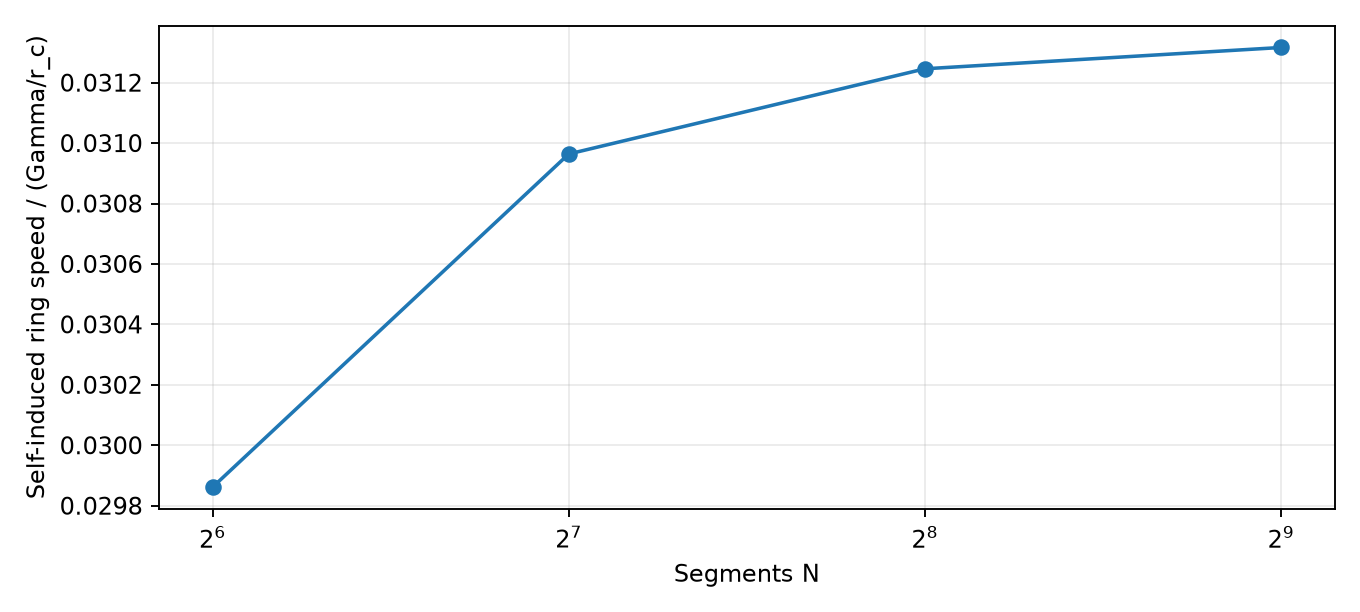
\includegraphics[width=.9\linewidth]{results/ring_convergence.png}\caption{Self-induced ring drift versus $N$ for a fixed regularization. Spatial refinement is not convergence of the continuous Euler model or of the core regulator itself.}\end{figure}

\section{SST-35: corrected spectral overlap and independent diagnostics}
SST-35 posits the unnormalized Gaussian drive and Lorentzian response \cite{SST35}:
\begin{equation}
S_d(\omega)=A\exp[-(\omega-\omega_0)^2/(2\sigma^2)],\quad
L(\omega)=\sum_n B_n\frac{\gamma_n^2}{(\omega-\omega_n)^2+\gamma_n^2}.
\end{equation}
If $V_{\rm norm}(\Delta;\sigma,\gamma)$ is the normalized, unit-integral Voigt line shape, where $\Delta=\omega_0-\omega_n$,
\begin{equation}
V_{\rm norm}=\frac{\Re w[(\Delta+i\gamma)/(\sigma\sqrt2)]}{\sigma\sqrt{2\pi}},\qquad
\boxed{Y=\int S_d L\,\dd\omega=A\sum_n B_n (\sqrt{2\pi}\sigma)(\pi\gamma_n)V_{\rm norm}(\Delta_n;\sigma,\gamma_n).}
\end{equation}
The factor $(\sqrt{2\pi}\sigma)(\pi\gamma_n)$ is essential when $A$ and $B_n$ are the original \emph{peak amplitudes} in SST-35. It may be absorbed in redefined line strengths, but cannot simply be omitted while holding the peak amplitudes fixed. The package compares the formula to direct numerical quadrature for multiple widths and detunings.

For a parameter vector $\theta=(\omega_1,\gamma_1,B_1)$ and Gaussian observational errors $\sigma_\epsilon$, the Fisher information is
\begin{equation}
\mathcal I(\theta)=\frac1{\sigma_\epsilon^2}\sum_k(\nabla_\theta Y_k)(\nabla_\theta Y_k)^T.
\end{equation}
One synthetic scan with multiple drive bandwidths gives rank$(\mathcal I)=3$ and condition number $163.88$; a noise-free fit retrieves the injected parameters $(0,0.35,1)$ with residual at floating-point precision. This demonstrates \emph{identifiability of the chosen fitting model}, not vortex eigenfrequency prediction. The $\omega_n$ here are injected test data, not measured PKLSA frequencies.
\begin{figure}[H]\centering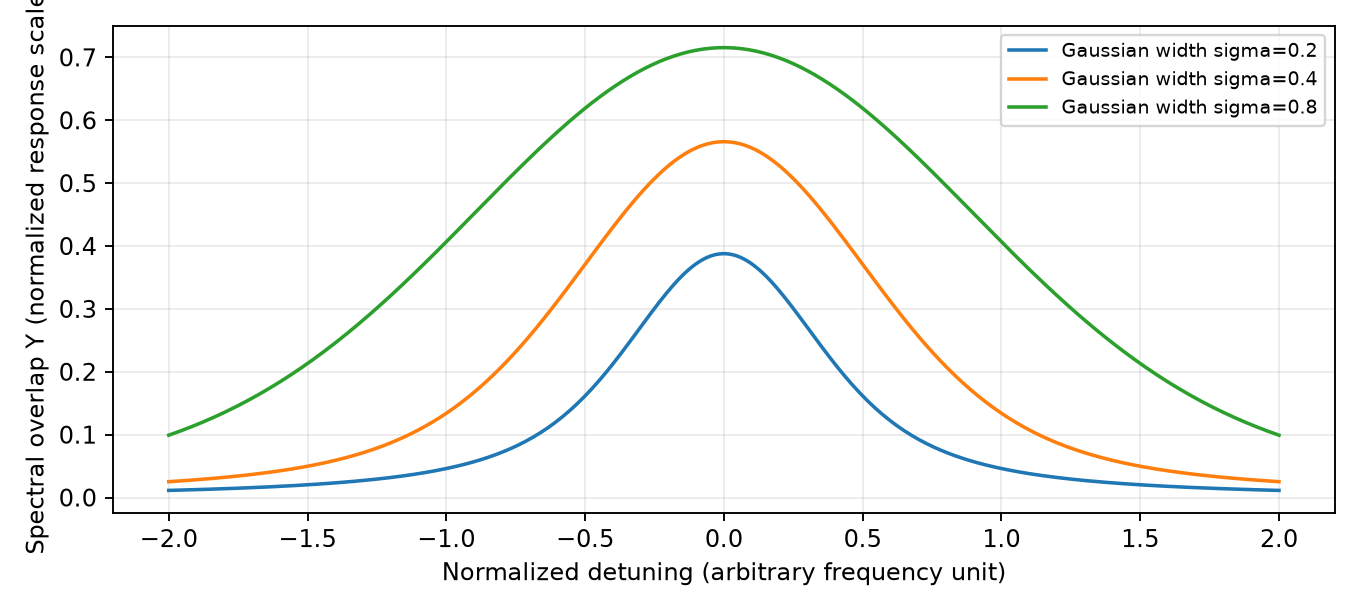
\includegraphics[width=.9\linewidth]{results/voigt_overlap.png}\caption{Illustrative normalized-unit overlap for one synthetic line and three source bandwidths. None of these curves are PKLSA modal spectroscopy.}\end{figure}

\section{SST-33: operational energetic tests, not thermodynamic closure}
The transport manuscript adapts off-diagonal mode coherences to a Lorentzian form $\gamma/(4\delta^2+\gamma^2)$, with $\delta,\gamma$ in $\mathrm{rad\,s^{-1}}$ \cite{SST33heat}. A measured thermal conductivity must have units $\mathrm{W\,m^{-1}\,K^{-1}}$. The cited schematic mode sum does not by itself establish that dimension without state normalization, mode density, energy factors, and sample geometry. The Born--Markov damping is a separate assumption that cannot be inserted into the conservative Euler action without an explicit reservoir and energy budget.

The paper's one-dimensional bar relation is dimensionally valid:
\begin{equation}
\Delta T=\frac{PL}{\kappa A_{\rm cross}},\qquad
\delta(\Delta T)=\frac{PL}{A_{\rm cross}}\left[\frac1{\kappa+\delta\kappa}-\frac1\kappa\right]
\simeq-\Delta T\,\frac{\delta\kappa}{\kappa}.
\end{equation}
At $P=20\ \mathrm{mW}$, $L=50\ \mathrm{mm}$, $A_{\rm cross}=10^{-4}\ \mathrm{m^2}$ and $\kappa=1.1\ \mathrm{W\,m^{-1}K^{-1}}$, $\Delta T=9.0909$ K. An \emph{assumed}, not calculated, $\delta\kappa/\kappa=-0.02$ gives a shift $+0.18553$ K. The document's $\sim0.18$ K benchmark is therefore arithmetically supported only \emph{conditional on the 2\% coupling}. A sign-reversing chiral asymmetry cannot be inferred from a scalar even-in-detuning line shape without a microscopic parity-odd interaction and independent null controls.

The separate SST-33 comparison defines the geometric strain $\epsilon=(r-\rc)/\rc$ and a proposed $T_{\rm swirl}=\Theta\epsilon$ \cite{SST33compare}. Its harmonic candidate is
\begin{equation}
\Delta E_{\rm strain}=\tfrac12K_{\rm eff}\epsilon^2
=\tfrac12\frac{K_{\rm eff}}{\Theta^2}T_{\rm swirl}^2,\qquad
\frac{\dd E_{\rm strain}}{\dd T_{\rm swirl}}=\frac{K_{\rm eff}}{\Theta^2}T_{\rm swirl}.
\end{equation}
The last derivative is an operational strain-energy slope; it is \emph{not automatically the equilibrium heat capacity} $C_V=(\partial\langle E\rangle/\partial T)_{V}$. Classical equilibrium statistical mechanics of one harmonic mode instead gives a constant high-temperature heat capacity; the quantum limit of a gapped harmonic oscillator is exponentially activated. Any claimed $C_V\propto T$ requires an independent density of states, population statistics and calibration of thermodynamic $T$. The Golden-layer log-periodic potential and clock-rate/temperature connection are not forced by Euler and are omitted from dynamical qualification.

\section{Falsification gates, baseline controls and native integration contract}
\begin{longtable}{p{.08\linewidth}p{.57\linewidth}p{.27\linewidth}}\toprule Gate&Acceptance/intent&v0.3.0 result\\\midrule\endhead
G0 & Canonical symbols, source trace, source hashes and dimensional distinctions & PASS documentation \\
G1 & v0.2.0 analytic/variational/free-director baseline, unmodified regression & PASS 47/47 \\
G2 & $0_1$/$3_1$ surrogate geometry, regularized velocity, impulse, RK4 short-time refinement & PASS \emph{surrogate only} (55-test suite) \\
G3 & Voigt integral vs quadrature, full-rank synthetic Fisher/fit checks & PASS \emph{synthetic only} \\
G4 & Thermal-bar dimensional arithmetic; strain temperature not conflated with $C_V$ & PASS \emph{formula audit only} \\
G5 & Registered PKLSA source module, engine commit/hash, model choices, XYZ provider and seed lineage & \NotRun / BLOCKED \\
G6 & Native PKLSA: independent modes for $N=1200,2400$ BASIC and $4800,9600$ FULL; space/time convergence with constant horizon; Swirl-Clock mode phase & \NotRun \\
G7 & Full coupled 3D Euler--director time evolution; independent EM, gravity, thermal and clock closure & UNRESOLVED\\\bottomrule\end{longtable}

For G5, use the canonical SST-Workbench provider rather than installing or inventing a competing PKLSA backend. The explicitly optional $\texttt{src/check\_native\_provenance.py}$ validates a manifest and SHA-256 of an externally supplied XYZ file; \emph{this is not an execution of the native physics}. The registered provider must specify source commit, finite-core regularization, coordinate units (meters or $r_c$), arclength convention, temporal integrator, boundary conditions, native threading/GPU backend, plus the fixed test horizon and a suite-specific science contract. Existing A001/A002/A003/A004 knot sources, E009/E010/E011 seed atlas files, and C005 dynamics are candidates for external selection, \emph{not}\, claimed as inspected or integrated here.

Native measurements should compute: vortex velocity fields and their divergence; pressure--Poisson consistency; circulation and helicity under explicit core conventions; line geometry and topology; total fluid energy and impulse; phase and frequency of at least two physically separable linearized response modes; freely predicted forced response versus withheld trajectories; and clock-ratio comparisons \emph{only after} the independent mode identification. Any finite nonzero inferred torsional wave speed remains unresolved until a mechanical wave sector is obtained from those native equations rather than fitted director stiffness.

\section{Conclusions and limits of the result}
The physical achievement of v0.3.0 is \emph{not} a new Maxwell or gravitational derivation: it is a reproducible separation of geometric motion, spectral measurement mathematics and tentative thermodynamic phenomenology. In the explicit surrogate, the ring advances axially, the trefoil has finite measured self-induced velocity and small short-time drift, and Voigt fitting is numerically identifiable with the corrected normalization. These do not establish the existence of a non-dissipative torsion photon, quantitative heat-capacity law or vortex-generated time dilation. The minimal next justified upgrade is \emph{G5/G6 native-PKLSA source and dynamics integration}; G7 can be considered only after native qualification.

\begin{thebibliography}{99}
\bibitem{VAM5} O. Iskandarani, \emph{On a Vortex-Based Lagrangian Unification of Gravity and Electromagnetism} (2025), Zenodo, \href{https://doi.org/10.5281/zenodo.15772858}{doi:10.5281/zenodo.15772858}.
\bibitem{SST17} O. Iskandarani, \emph{Electromagnetism as Propagating Torsion in a Hydrodynamic Vacuum} (2026), Zenodo, \href{https://doi.org/10.5281/zenodo.17677074}{doi:10.5281/zenodo.17677074}.
\bibitem{SSTv020} SST Research Workbench, \emph{VAM-5 $\times$ SST-17 Integrated Euler--Director Action v0.2.0}, research report (2026), DEVELOPMENT.
\bibitem{SST33heat} O. Iskandarani, \emph{Coherence-Enhanced Heat Transport and Entropy Production in 1D: Predictions and Falsifiers} (2026), Zenodo, \href{https://doi.org/10.5281/zenodo.17459746}{doi:10.5281/zenodo.17459746}.
\bibitem{SST33compare} O. Iskandarani, \emph{Comparative Thermodynamics of Topological Defects and Quantum Ensembles} (2026), Zenodo, \href{https://doi.org/10.5281/zenodo.18388722}{doi:10.5281/zenodo.18388722}.
\bibitem{SST35} O. Iskandarani, \emph{Resonance-Matched Excitation: A General Overlap Model for Beam--Target Spectroscopy, Identifiability, and Optimal Design}, manuscript (2026); its displayed DOI is a placeholder, not a verified identifier.
\bibitem{Saffman} P. G. Saffman, \emph{Vortex Dynamics}, Cambridge University Press (1992), ISBN 9780521420587.
\bibitem{AllenFeldman} P. B. Allen and J. L. Feldman, ``Thermal conductivity of disordered harmonic solids,'' \emph{Phys. Rev. B} \textbf{48}, 12581 (1993), \href{https://doi.org/10.1103/PhysRevB.48.12581}{doi:10.1103/PhysRevB.48.12581}.
\bibitem{Simoncelli} M. Simoncelli, N. Marzari and F. Mauri, ``Unified theory of thermal transport in crystals and glasses,'' \emph{Nature Physics} \textbf{18}, 1180 (2022), \href{https://arxiv.org/abs/1901.01964}{arXiv:1901.01964}.
\bibitem{AbeOkuyama} S. Abe and S. Okuyama, ``Similarity between quantum mechanics and thermodynamics: Entropy, temperature and Carnot cycle,'' \emph{Phys. Rev. E} \textbf{83}, 021121 (2011), \href{https://doi.org/10.1103/PhysRevE.83.021121}{doi:10.1103/PhysRevE.83.021121}.
\bibitem{Weideman} J. A. C. Weideman, ``Computation of the complex error function,'' \emph{SIAM J. Numer. Anal.} \textbf{31}, 1497--1518 (1994), \href{https://doi.org/10.1137/0731077}{doi:10.1137/0731077}.
\end{thebibliography}
\end{document}
